\documentclass[class=book, crop=false, oneside, 12pt]{standalone}
\usepackage{standalone}
\usepackage{../../style}
\usepackage[normalem]{ulem}
\graphicspath{{./assets/images/}}

% arara: pdflatex: { synctex: yes, shell: yes }
% arara: latexmk: { clean: partial }
\begin{document}
\chapter[Parsing bottom-up: LR(1) e LALR(1)]{Analisi sintattica: parsing bottom-up LR(1) e LALR(1)}

\section{L'automa caratteristico LR(1)}
Riprendiamo il filo del discorso: nel precedente capitolo siamo andati a discutere tutti i passaggi che, partendo da una grammatica, ci conducono ad eseguire il parsing bottom-up. Consigliamo di tornare a dare un occhio allo schema presentato in \autoref{subsec:schema}. Ci eravamo lasciati con una questione alquanto spinosa: avevamo constato che è possibile ritrovarsi con due reducing items in uno stesso stato anche se la grammatica di partenza non è ambigua, e questa situazione potrebbe essere risolta conservando, per ogni stato, delle informazioni rispetto a quali simboli potrebbero seguirgli in lettura. Ci eravamo resi conto di non aver modo di conservare e impiegare efficacemente queste informazioni con la tecnica di costruzione dell'automa SLR(1), il che lascia pensare solo a una cosa: è il momento di abbandonare questa tecnica e guardare a soluzioni più complesse, certo, ma senza dubbio più efficaci. È il momento di affrontare la costruzione di un automa caratteristico LR(1).
\subsection{Stati}
\paragraph{Gli LR(1)-items}
Per prima cosa dobbiamo ricordarci che la principale differenza sta proprio in cosa popola gli stati dei diversi automi: per gli automi SLR(1) utilizzavamo gli LR(0)-items, gli automi LR(1) invece utilizzano gli LR(1)-items.
\paragraph{Forma}
Gli LR(1)-items hanno questa forma:
\begin{equation}
    \label{lr0}
    [A \to \alpha \cdot B \beta, \Delta]
\end{equation}
Possiamo vedere subito che un LR(1)-item è una tupla di due elementi:
\begin{enumerate}
    \item il primo è un LR(0)-item \((A \to \alpha \cdot B \beta)\);
    \item il secondo è un insieme di caratteri \((\Delta)\) detto \textbf{lookahead set}.
\end{enumerate}

\subsection{Chiusura di un insieme di LR(1)-item}
Quando andiamo a calcolare la chiusura di un item di tipo LR(1) utilizziamo la \(closure_1(item)\) e non la \(closure_0(item)\), che funziona esattamente come la \(closure_0\) ma in più ci permette di aggiornare l'insieme \(\Delta\), il lookahead set. Questo insieme ci torna poi utile quando dobbiamo inserire mosse di riduzione in qualche stato dell'automa caratteristico LR(1): il lookahead set specifica quali caratteri ci dobbiamo aspettare di vedere in lettura quando stiamo per utilizzare una mossa di reduce.

\paragraph{Funzionamento}
Ma specifichiamo ora meglio come è strutturata l'operazione di \(closure_1(item)\):
\begin{itemize}
    \item la prima parte della chiusura è in tutto e per tutto uguale alla \(closure_0(item)\), quindi quando si calcola una \(closure_1(item)\) la prima cosa che si fa è appunto calcolare la \(closure_0(item)\), utilizzando la parte LR(0) dell'item LR(1) che stiamo chiudendo;
    \item la seconda parte prevede di aggiornare l'insieme di lookahead, che viene aggiunto alla \(closure_0(item)\) appena calcolata.  
\end{itemize}
Di fatto con questo metodo di calcolo l'informazione contenuta nell'insieme \(\Delta\) di un LR(1)-item viene tramandata agli item che ne derivano grazie alla seconda parte della procedura \(closure_1\), così se si segue una derivazione lungo tutto l'albero delle produzioni guardando a \(\Delta\) si ha sempre sotto controllo quali simboli ci si aspetta di leggere in un certo stato quando si deve effettuare una mossa di riduzione.

\paragraph{Calcolo}
Come facciamo a calcolare la chiusura degli insiemi di LR(1)-items? Il metodo di calcolo che ci viene presentato è un classico calcolo risolvibile grazie al teorema del punto fisso:
\begin{definition}
    \label{def:lr1-closure}
    Sia \(P\) un insieme di LR(1)-item, la \(closure_1(P)\) identifica il più piccolo insieme di item, con il più piccolo lookahead-set, che soddisfa la seguente equazione:
    \begin{align*}
        closure_1(P) = P \; \cup \; &\{[B \rightarrow \cdot \gamma, \Gamma] : [A \rightarrow \alpha \cdot B \beta, \Delta] \in closure_1(P) \; \land \\ 
        & B \rightarrow \gamma \in \P' \; \land \\
        & first(\beta \Delta) \subseteq \Gamma\}
    \end{align*}  
    dove \(first(\beta \Delta) = \cup_{d \in \Delta} first(\beta d)\) e ricordiamo che \(\P'\) è ricavato dall'insieme delle produzioni \(\P\) aggiungendo la produzione \(S' \to S\).
\end{definition}
\paragraph{Algoritmo}
Dal momento che la Def.\ref{def:lr1-closure} non risponde molto bene al richiamo degli attributi "semplice e intuitiva", potrebbe essere una buona idea dare un'occhiata alla sua formulazione algoritmica in Alg.\ref{alg:lr1-closure}. \\
% \begin{figure}[H]
%     \centering
%     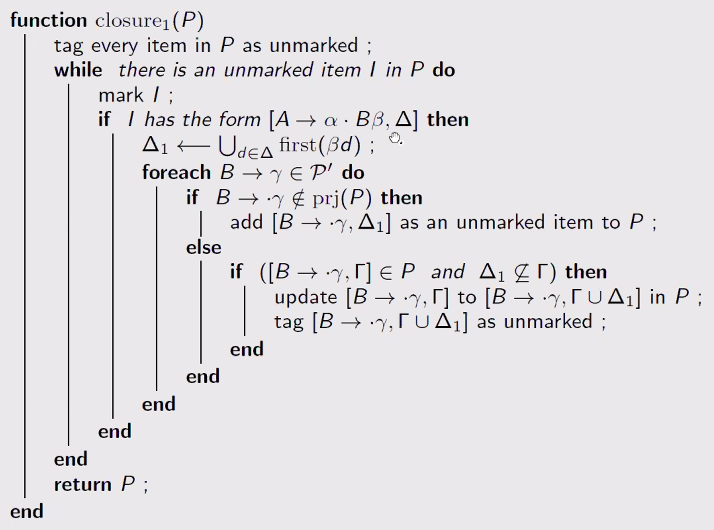
\includegraphics[width=\textwidth,keepaspectratio]{alg_closure-lr1.png}
%     \caption{Algoritmo per il calcolo della chiusura di uno stato LR(1)}
%     \label{alg:closure-lr1}
% \end{figure}
\subimport{assets/pseudocode/}{lr1-closure.tex}
In questo algoritmo si deve fare conto che \(B \to \cdot \gamma \notin prj(P)\) significa che non è ancora presente in \(closure_1(P)\) una produzione \(B \to \cdot \gamma\).
Di fatto quello che succede all'interno del \texttt{foreach} centrale è che se l'elemento è nuovo vado ad aggiungerlo con il suo \(\Delta\), se l'elemento è già presente vado a vedere se è il caso di aggiungere al \(\Delta\) di questa qualche elemento. Il procedimento potrebbe risultare un po' ostico, ma sarà tutto più chiaro dopo qualche esercizio esplicativo, come al solito.

\subsubsection{Esercizio di calcolo di \(closure_1(P)\)}
Facendo riferimento alla grammatica dell'esercizio precedente (riportata qui sotto), calcolare tutti gli stati dell'automa caratteristico LR(1).
\begin{align}
    \label{eq:ex3-slr1-grammarr}
    \G: S &\to aAd \mid bBd \mid aBe \mid bAe \\
    A &\to c \nonumber \\ \notag
    B &\to c \notag
\end{align}
\paragraph{Descrizione della procedura per lo stato 0}
Partiamo con l'inizializzazione dello stato \(0\), che conterrà la \(closure_1(\{[S' \to \cdot S, \{\$\}]\})\); questa inizializzazione sottolinea il fatto che, che una volta che avremo raggiunto il particolare stato in cui avremo l'accepting item \(S' \to S\cdot \), vorremo vedere il \$ che viene utilizzato come terminatore per definire una parola appartenente al linguaggio. Quindi, che si fa ora?

Secondo la Def.\ref{def:lr1-closure}, la \(closure_1(P)\) va inizializzata con \(P\) stesso, ovvero \([S' \to \cdot S, \{\$\}]\).
In seguito dobbiamo andare a prendere, all'interno della \(closure_1(P)\) (che è parziale, non ancora completa), tutti gli elementi in forma \([A \rightarrow \alpha \cdot B \beta, \Delta]\) e dovremo aggiungere alla stessa \(closure_1(P)\) tutti quegli item che soddisfano la forma \([B \rightarrow \cdot \gamma, \Gamma]\), dove \(\Gamma\) è un insieme calcolato come descritto dall'algoritmo; niente paura, in seguito sarà tutto più chiaro.

Nel nostro caso l'unico item in \(closure_1(P)\) è \([S' \to \cdot S, \{\$\}]\), che corrisponde alla forma desiderata (\([A \to a \cdot B\beta, \Delta]\)), quindi possiamo assumere \(\Delta = \{\$\} \textrm{ e } \beta = \varepsilon\); di conseguenza, \(first(\varepsilon \$) = first(\$) = \{\$\} \subseteq \Gamma\). Gli item che otteniamo da \(closure_1(\{[S' \to \cdot S, \{\$\}]\})\) saranno dunque:
\begin{align*}
    [&S' \to \cdot S, \{\$\}] \\
    [&S \to \cdot aAd, \{\$\}] \\
	[&S \to \cdot bBd, \{\$\}] \\
	[&S \to \cdot aBe, \{\$\}] \\
	[&S \to \cdot bAe, \{\$\}]
\end{align*}
Quanto abbiamo appena ottenuto è la chiusura dell'insieme che costituisce lo stato 0 del nostro automa caratteristico di tipo LR(1).
Come già detto prima, la prima parte di questi item è esattamente corrispondente all'item LR(0) che avremmo trovato utilizzando SLR parsing, la seconda parte (ovvero il \(\Delta\)) è l'unica novità introdotta dalla procedura LR(1).

\paragraph{Iterazione della procedura sulle transizioni}
È da notare anche che la componente del lookahead-set è usata solo in caso di riduzioni, e non incide sulle transizioni, per cui il procedimento rimarrà sotto quel punto di vista inalterato rispetto al metodo SLR. Di conseguenza, possiamo affermare la presenza, di tre transizioni che portano a tre stati differenti: \(\tau(0,S)=1 \textrm{, } \tau(0,a)=2 \textrm{ e } \tau(0,b)=3\). A questo punto è possibile procedere come abbiamo sempre fatto, prestando attenzione al calcolo della \(closure_1(S)\):
\begin{enumerate}
    \item Proseguiamo osservando lo stato \(\tau(0, S)=\)1. Il suo kernel è:
    \begin{equation*}
        [S' \to S \cdot, \{\$\}]
    \end{equation*}
    dobbiamo dunque calcolare \(closure_1(\{[S' \to S \cdot, \{\$\}]\})\), per cui sappiamo che \(B = \varepsilon\) e dunque non possiamo fare altro se non appuntarci che lo stato 1 contiene l'Accepting Item.
    \item Analizziamo dunque lo stato \(\tau(0, a)=\)2, il cui kernel è popolato da questi item:
    \begin{align*}
        [S &\to a \cdot Ad, \{\$\}] \\
        [S &\to a \cdot Be, \{\$\}]
    \end{align*}
    entrambi soddisfano la forma \([A \rightarrow \alpha \cdot B \beta, \Delta]\).
    Nel primo caso abbiamo le seguenti corrispondenze: \(A=S\), \(\alpha = a\), \(B = A\), \(\beta = d\) e \(\Delta=\$\); andiamo a cercare nella nostra grammatica se sono presenti derivazioni in forma \(B \to \gamma\). Troviamo \(A \to c\), quindi grazie alla formula del calcolo di \(closure_1(P)\) sappiamo che dobbiamo aggiungere agli item dello stato 2 un item formato così: \([A \to \cdot c, {\Gamma}]\), dove \(\Gamma = first(\beta\Delta) = first(d\$) = \{d\}\); in definitiva, aggiungiamo l'item \(A \to \cdot c, \{d\}\).

    Abbiamo detto che anche la seconda produzione (\([S \to a \cdot Be, \{\$\}]\)) soddisfa la forma \([A \rightarrow \alpha \cdot B \beta, \Delta]\), quindi con lo stesso procedimento appena adottato possiamo trovare la chiusura di \([S \to a \cdot Be, \{\$\}]\): in questo caso le corrispondenze sono: \(A=S\), \(\alpha=a\), \(B=B\), \(\beta=e\) e \(\Delta=\$\), la produzione da analizzare è \(B \to c\) e l'item che ne ricaviamo è \([B \to \cdot c, {\Gamma}]\), dove \(\Gamma = first(\beta\Delta) = first(e\$) = \{e\}\).
    
    In sostanza, lo stato 2 contiene questi LR(1) items:
    \begin{align*}
        [S &\to a \cdot Ad, \{\$\}] \\
        [S &\to a \cdot Be, \{\$\}] \\
        [A &\to \cdot c, \{d\}] \\
        [B &\to \cdot c, \{e\}]
    \end{align*}
    Come succedeva nell'esempio con il parsing LR(0), nello stato 2 possiamo osservare la presenza di tre transizioni e quindi di tre possibili nuovi stati che sono \(\tau(2,A)=4 \textrm{, } \tau(2,B)=5 \textrm{ e } \tau(2,c)=6\).
    \item[...]
    \item[6.] Ovviamente la parte interessante dell'esercizio è verificare se siamo riusciti a risolvere il conflitto che occorreva nel parsing SLR(0). In modo pressoché analogo a quanto accadeva, abbiamo che il kernel per lo stato 6 è :
    \begin{align*}
        [A &\to c \cdot, \{d\}] \\
        [B &\to c \cdot, \{e\}]
    \end{align*}
    Anche questa volta nello stato sono presenti due item di riduzione, ma non troviamo più il conflitto che avevamo con il parsing LR(0), perché in questo caso la riduzione \(A \to c\) si applica solo se nell'input buffer si sta leggendo \(d\), mentre la riduzione \(B \to c\) si applica solo nel caso in cui nell'input \emph{buffer} si sta leggendo \(e\). Questo implica che nello stato 6, grazie al parsing LR(1), è stata eliminata l'ambiguità del conflitto r/r.
\end{enumerate}

\subsubsection{Facciamone un altro, dai}
\label{ex:closure-lr1}
Sia data la seguente grammatica:
\begin{align}
    \G: S &\to L=R \mid R \\
    L &\to *R \mid id \nonumber \\ \notag
    R &\to L \notag
\end{align}
Inizializziamo lo stato 0 ponendo come suo kernel:
\begin{equation*}
    [S' \to \cdot S, \{\$\}]
\end{equation*}
Calcoliamo \(closure_1(0)\). Questo item soddisfa la forma \([A \rightarrow \alpha \cdot B \beta, \Delta]\), con le seguenti corrispondenze: \(B = S \texttt{, } \beta = \varepsilon \texttt{, } \Delta = \{\$\}\) (e quindi \(\Gamma = first(\beta \Delta) = first(\varepsilon \$) = \{\$\}\)).
Le due produzioni di \(B\) (ovvero di \(S\)) in questo caso sono \(S \to L=R \mid R\), quindi aggiungo i due item LR(1) seguenti:
\begin{align}
    \label{prod:production-L}
    [S &\to \cdot L = R, \{\$\}] \\
    [S &\to \cdot R, \{\$\}] \notag
\end{align}
A questo punto la chiusura non è completa in quando abbiamo aggiunto due elementi che possono essere presi in considerazione nella definizione ricorsiva della chiusura, ovvero soddisfano anch'essi la famosa forma \([A \rightarrow \alpha \cdot B \beta, \Delta]\).
Analizziamo dunque \([S \to \cdot L = R, \{\$\}]\), le sue corrispondenze sono: \(B = L \texttt{, } \beta = \; \; =R \texttt{, } \Delta = \{\$\}\) (e quindi \(\Gamma = first(\beta \Delta) = first(=R\$) = \{=\}\)); le produzioni di \(L\) sono \(L \to *R \mid id\), quindi arriviamo a generare i seguenti LR(1)-items:
\begin{align*}
    [L &\to \cdot *R, \{=\}] \\
    [L &\to \cdot id, \{=\}]
\end{align*}
che non presentano altre possibili espansioni (grazie al cielo).

Ci rimane ora da analizzare \([S \to \cdot R, \{\$\}]\), che soddisfa la nostra formosa forma e presenta le seguenti corrispondenze: \(B = R \texttt{, } \beta = \{\varepsilon\} \texttt{, } \Delta = \{\$\}\) (e quindi \(\Gamma = first(\beta \Delta) = first(\varepsilon \$) = \{\$\}\)), inoltre le produzioni di \(R\) sono \(R \to L\), quindi otteniamo il seguente LR(1)-items:
\begin{align*}
    [R &\to \cdot L, \{\$\}]
\end{align*}
questo item presenta il marker davanti a un non-terminale; può generare nuovi item per la chiusura che stiamo calcolando?
Nonostante la produzione con driver \(L\) sia già stata analizzata (vedi Eq.\ref{prod:production-L}), è necessario eseguire nuovamente la sua chiusura in quanto ha un lookahed-set differente (nel caso precedente \(\beta= \; \;  =R\), mentre ora \(\beta=\varepsilon\)), il che ci porta a ripetere la chiusura per l'item \([R \to \cdot L, \{\$\}]\), ricavando i seguenti LR(1)-items:
\begin{align*}
    [L &\to \cdot *R, \{\$\}] \\
    [L &\to \cdot id, \{\$\}]
\end{align*}
Visto che però avevamo già inserito due LR(1)-item con lo stesso LR(0)-item (la parte \(L \to \cdot qualcosa\)) possiamo semplicemente accrescere i lookahead-set corrispondenti. Il risultato finale per la chiusura degli item dello stato iniziale è:
\begin{align*}
    [&S'\to \cdot S, \{\$\}] \\
    [&S \to \cdot L = R, \{\$\}] \\
    [&S \to \cdot R, \{\$\}] \\
    [&L \to \cdot *R, \{\$, =\}] \\
    [&L \to \cdot id, \{\$, =\}] \\
    [&R \to \cdot L, \{\$\}]
\end{align*}
Bene, ora abbiamo fatto un po' di allenamento con il calcolo degli stati, ma dobbiamo ricordare che non è questo il nostro obiettivo finale, noi vogliamo ricavare l'automa caratteristico!

\subsection{Costruzione di un automa caratteristico LR(1)}
Partiamo spiegando il modo più semplice per costruire un automa caratteristico LR(1):
\begin{enumerate}
    \item costruiamo lo stato di partenza con l'item \([S' \to \cdot S, {\$}]\);
    \item ricorsivamente aggiungiamo gli stati che si possono raggiungere dagli stati presenti nell'automa;
    \item aggiungamo le transizioni che ci permettono di passare da uno stato all'altro.
\end{enumerate}
E come facciamo a capire quali stati sono collegati ad un certo stato \(P\)?

\noindent Se uno stato \(P\) contiene un item nella forma \([A \to \alpha \cdot Y \beta, \Delta]\) allora esiste una transizione da \(P\) ad uno stato \(Q\) che contiene l'item \([A \to \alpha Y \cdot \beta , \Delta]\); inoltre, siccome \(Q\) contiene \([A \to \alpha Y \cdot \beta , \Delta]\), esso contiene anche tutti gli item in \(closure_1([A \to \alpha Y \cdot \beta , \Delta])\).

Proviamo ora a chiarire tale procedura tramite la sua scrittura in forma algoritmica, si veda \ref{alg:lr1-automata}.

% \begin{figure}
%     \centering
%     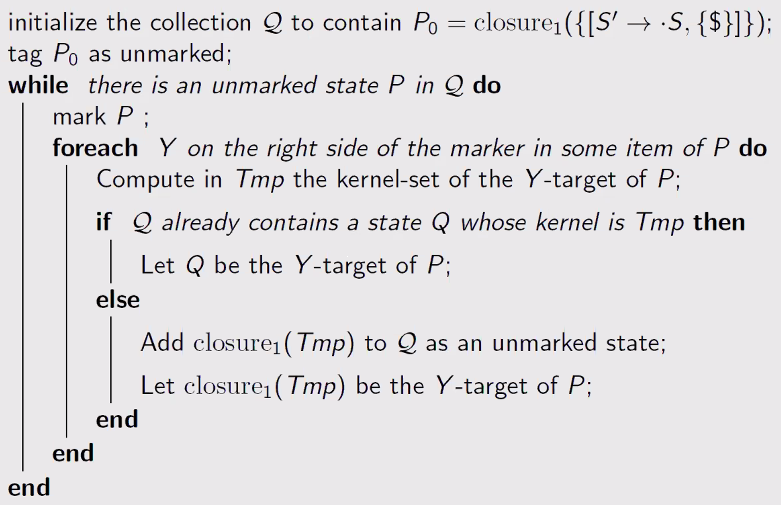
\includegraphics[width=\textwidth]{alg-construct-lr1-automata.png}
%     \caption{Algoritmo per la costruzione di un automa LR(1)}
%     \label{alg:construct-lr1-automata}
% \end{figure}
\subimport{assets/pseudocode/}{lr1-automata.tex}
Indovinate un po' con quale grammatica stiamo per andare a osservare cosa si ottiene con questa procedura? Oh sì! proprio lei:
\begin{align}
    \label{eq:ex3-slr1-grammarrrrrr-again-and-again}
    \G: S &\to aAd \mid bBd \mid aBe \mid bAe \\
    A &\to c \nonumber \\ \notag
    B &\to c \notag
\end{align}
Ora chiederemo al lettore di fare uno sforzo mnemonico poderoso e di ricordare che in passato, quando abbiamo provato a costruire l'automa caratteristico di tipo SLR per questa grammatica ci siamo trovati ad avere la situazione rappresentata in figura \ref{fig:lr0-automata_conflict}, che riprtiamo qui sotto per comodità.
\begin{figure}[H]
    \centering
    \subimport{assets/figures/}{automa_conflict_LR.tex}
    \caption{Automa di tipo LR(0), si noti il conflitto sullo stato 6}
    \label{fig:lr0-automata_conflict}
\end{figure}
Abbiamo già calcolato quali sono gli stati LR(1) per la grammatica in questione in un esercizio precedente (vedi \ref{ex:closure-lr1}), ed applicando l'algoritmo per la costruzione degli automi LR(1) arriviamo ad ottenere il seguente automa (parziale):
\begin{figure}[H]
    \centering
    \subimport{assets/figures/}{automa_conflict_solution_LR.tex}
    \caption{Automa di tipo LR(1), si noti che il conflitto sullo stato 6 è stato eliminato}
    \label{fig:lr1-automata_no-conflict}
\end{figure}
Ma siamo sicuri di aver effettivamente risolto il problema? per verificarlo dobbiamo costruire la parsing table!

La costruzione della parsing table per il parsing di tipo LR(1) è semplice da ottenere perché si crea esattamente come la parsing table per l'SLR parsing con queste uniche due differenze:
\begin{itemize}
    \item l'automa caratteristico è di tipo LR(1);
    \item la lookahead function utilizzata è la seguente: per ogni \([A \to \beta \cdot , \Delta] \in P\), \(\mathcal{LA}(P, A \to \beta ) = \Delta\).
\end{itemize}
Naturalmente una grammatica \(\mathcal{G}\) è di tipo LR(1) se la sua tabella di parsing LR(1) non presenta conflitti.

Sbirciamo quindi cosa sarebbe successo costruendo la parsing table LR(1) per la nostra grammatica preferita.

Innanzitutto, l'automa caratteristico LR(1) si presenta come in Fig.\ref{fig:lr1_automata-complete}
\begin{figure}[H]
    \centering
    \subimport{assets/figures/}{automa_LR_complete_solution.tex}
    \caption{Automa di tipo LR(1) completo}
    \label{fig:lr1_automata-complete}
\end{figure}
Negli stati 6 e 9, che ci avrebbero causato problemi con la costruzione di tipo LR(0), ora troviamo i seguenti item:
\begin{itemize}
    \item Stato 6
    \begin{align*}
        A &\to c \cdot , {d} \\
        B &\to c \cdot , {e}    
    \end{align*}
    \item Stato 9
    \begin{align*}
        A &\to c \cdot , {e} \\
        B &\to c \cdot , {d}    
    \end{align*}
\end{itemize}
 Quindi, seguendo le regole di compilazione della tabella di parsing LR(1) avremmo:
 \begin{itemize}
     \item nella casella M[6,d] la riduzione \(A \to c \cdot , {d}\);
     \item nella casella M[6,e] la riduzione \(B \to c \cdot , {e}\);
     \item nella casella M[9,e] la riduzione \(A \to c \cdot , {e}\);
     \item nella casella M[9,d] la riduzione \(B \to c \cdot , {d}\);
 \end{itemize}
Festa! Festa! non ci sono più conflitti!
È però notevole il fatto che il numero di stati sia aumentato parecchio: questo è quello che succede quando si va ad utilizzare tecniche di parsing più precise e raffinate.

\section{Costruzione di una tabella di parsing LR(1)}
\subsection{Esercizi: costruzione di parsing table LR(1)}
Mettiamoci ora di buona lena ad esercitarci con la costruzione di tabelle di parsing di tipo LR(1).

\subsubsection{Esercizio 1}
La prima grammatica che andiamo ad analizzare è la seguente:
\begin{align}
    \label{gr:pointers-grammar}
    S &\to L = R \mid R \\
    L &\to *R \mid id \nonumber \\ \notag
    R &\to L \notag
\end{align}
Questa è una grammatica che ci parla di puntatori, ma capiremo in seguito cos significa ciò, per ora concentriamoci sulla sua risoluzione.

È il momento di campiare Pokémon, vai DaPips, scelgo te!


\section{SPOILER: TUTTO QUELLO CHE SEGUE È UNA LEZIONE NON SCRITTA}

Ripartiamo dalla risoluzione dell'esercizio di ieri.
Avevamo già osservato tutti gli stati da 0 a 5, riportiamoli qui:
\begin{figure}[H]
    \centering
    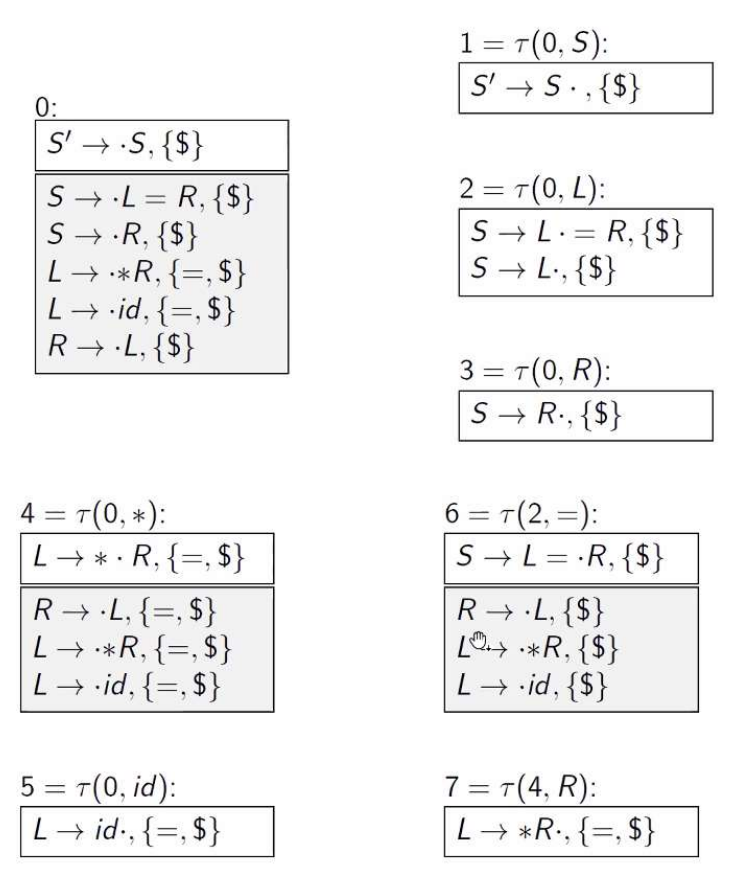
\includegraphics[width=.8\textwidth]{send_help_1.png}
    \caption{help}
\end{figure}
Descrizione degli stati?
Lo stato 7:
Il kernel dello stato 7 non presenta possibilità di chiusura, ma conterrà riduzione, passiamo oltre.
\begin{figure}[H]
    \centering
    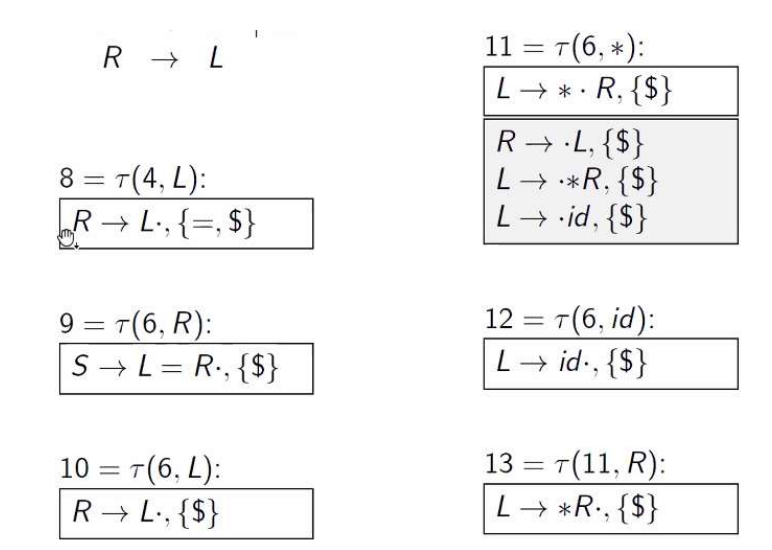
\includegraphics[width=.8\textwidth]{send_help_2.png}
    \caption{help}
\end{figure}
Per tutti gli stati 8,9 e 10 non ci sono chiusure ma si presentano riduzioni.
Nello stato 11 il kernel permette di cercare una chiusura per R, la chiusura per R ci porta a R -> .L, {\$}
che ci permette un'ulteriore chiusura, con conseguente inserimento di L->.*R,{\$} e L->.id,{\$}.
Passiamo allo stato 12 ha un kernel che potrebbe sembrare uguale allo stato 5, ma il lookahead set è
diverso… quindi lo stato 12 è diverso dal 5
Aggiungiamo anche lo stato 13 per rappresentare la transizione \(\tau(11,R)\) ecc. ecc.
Nota che la Quaglia non ha riportato tutti gli stati ed i relativi items.
Questo è l'automa che ricaviamo:
\begin{figure}[H]
    \centering
	\subimport{assets/figures/}{figures_9-7.tex}
    \caption{help}
\end{figure}
Ora la domanda diventa: questa grammatica è LR(1)?
Potremmo ripsondere cosruendo la tbella di parsing e controllando che non vi siano conflitti.
\begin{figure}[H]
    \centering
    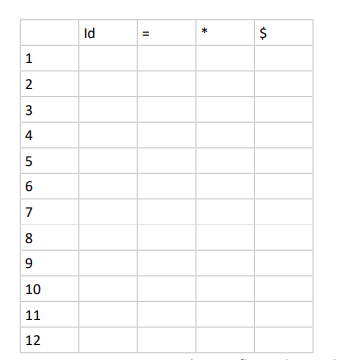
\includegraphics[width=.8\textwidth]{send_help_4.png}
    \caption{help}
\end{figure}
Oppure possiamo notare che i conflitti reduce-reduce non sono presenti, perché in nessuno stato
sono presenti due riduzioni: in nessuno stato è presente più di un item che porta riduzione.
Ma sono presenti conflitti shift reduce?
Come si verifica questo?
Si va a vedere tutti gli stati che presentano riduzioni (tutti quelli con il doppio cerchiolino
nel'automa) e si verifica che non presentino mosse di shift (frecce uscenti).
Gli stati 3,5,7,8, ecc. non presentano problemi perché non presentano shift.
Mentre lo stato 2 potrebbe presentare problemi dato che presenta sia riduzione che shift, ma
andando subito a verificare ci rendiamo conto che la riduzione viene applicata per \$ mentre lo shift
viene applicato per =, quindi festa festa non ci sono conflitti, la grammatica è LR(1).
Ora ci chiediamo invece se la grammatica è slr(1)?
Ricordiamo che la risoluzione di tipo SLR(1) prevede di utilizzare l'automa LR(0) e di utilizzare come 
lookahead function follow(B) ; in tal caso l'automa sarebbe stato il seguente:
\begin{figure}[H]
    \centering
	\subimport{assets/figures/}{figures_9-9.tex}
    \caption{help}
\end{figure}
E si sarebbe verificato un problema per lo stato 2, dato che avrebbe presentato uno shift per = ma
usando come lookahead function follow(B) avremmo inserito = anche come item valido per la
riduzione, quindi nella casella [2, = ] della tabella di parsing SLR(1) avremmo avuto un conflitto shiftreduce.
La grammatica quindi risulta essere LR(1) ma non SLR(1).
A che cosa gioca questa grammatica?

Abbiamo già detto in passato come questa sia una grammatica che ci parla di puntatori, andiamo ora
ad indagare più a fondo tale affermazione:

L sta per left
R sta per right

Notiamo che il non-terminale S si presenta una sola volta per derivazione, ed essendo l'unico che
genera = allora l'= può essere presente all'interno di una derivazione al massimo una volta.. Cosa
sappiamo del resto?

Che linguaggio possiamo ricavare da tale grammatica?
% {( (*)^n id ) = ( (*)^k id ), n,k>=0} U {(*)^n id, n>=0} forse
Continueremo questo discorso? Mah

Qui nel frattempo discutiamo di come in 5 si presenti una riduzione per id
\begin{figure}[H]
    \centering
	\subimport{assets/figures/}{figures_9-10.tex}
    \caption{help}
\end{figure}
Dato che lo stato 5 contiene l'elemento di riduzione
Voglio arrivare in 2, voglio capire come faccio ad arrivare in 2 e voglio capire perché qui ci sia un
conflitto.
Il 2 lo raggiungo tramite L dallo stato 0, L è un non terminale e non lo leggerò mai dall'input buffer, lo
leggerò per forza da un goto.
Devo quindi aver fatto una riduzione che mi riporta allo stato 0 e mi inserisce L nella pila dell'analisi.
Quindi una delle possibili riduzioni che ci portano allo stato 0 con L sulla pila dei simboli è la
riduzione in 5 per id.
Proviamo a capirlo facendo il parsing di "id = id"
Partiamo da 0, leggiamo id, ci spostiamo in 5.
In 5 esiste la riduzione L -> id.
Simboli: id
Stati: 0 5
Applico la riduzione
Simboli:
Stati: 0
Inserisco il driver della riduzione e mi muovo allo stato della transizione
Simboli: L
Stati: 0 2
Ora sono nello stato 2 e leggo =, ora trovo lo shift reduce conflict!
Ma qual è l'azione giusta da fare?
La riduzione è R->L non ha senso perché non ho mai letto un asterisco prima, quindi è sciocco
chiedersi se sia giusto applicare la riduzione R->L (siamo partiti da id=id ed abbiamo trasformato
subito la L derivata da S in id, senza mai passare da stringhe con *, quindi non sono mai passato da
produzioni R->L).
Proviamo ora con ***id = id
Qal'è il percorso che compio?
0 4 4 4 5, poi incontro la riduzione che mi mette L sui simboli ecc. ecc.
0 4 4 4 8
 * * * L(L->id)
Altra riduzione perché trovo in 8 la riduzione R->L
Sbam passo allo stato 7, dove
trovo una riduzione L->R
* * * R
0 4 4 7
Proced

Procedo così un po' di volte, quello che succede è che rimbalzo tra 8 e 7 fino a che non "assorbo"
(Quagliabolario) tutti gli asterischi, quindi ad un certo punto dopo l'ennesima soluzione m imangio
tutti gli stait 4 e arrivo allo stato 0
Nello stato 0 avrò un goto L che mi porterà nello stato 2 con coflitto annesso, cosa è giusto fare?
Shift o reduce per riconoscere la parola?
Proviamo con lo shift:
Mi sposto sullo stato 6 e consumo = in lettura
0 2 6
L =
ora vedo id, id mi porta in 5 che tramite riduzione L-> id mi sbatte nello stato 8
0 2 6 8
L = L
Ora trovo la riduzione di 8 R->L che mi sbatte in 9
0 2 6 9
L = R
In 9 trovo l'ennesima riduzione S -> L = R, comunque sia questa riduzione ci porta ad arrivare fino
all'accepting item quindi bingo.
Cosa sarebbe successo se una volta arrivati nello stato 2 avessimo scelto la mossa di reduce R->L?
Da 2 saremmo passati allo stato 3 con la seguente situazione:
0 3
Nello stato 3 noi leggiamo =, che non ha nessuna mossa corrispondente, quindi siamo finiti in una
casella error della tabella di parsing.
La scelta giusta era lo shift.
LALR
Le grammatiche LALR sono tali per cui la loro complessità in spazio (la dimensione della tabella) è
esattamente uguale a SLR ma la funzione di lookahead è ben più raffinata.
Mentre in SLR si va ad usare il follow(B), mentre in SLR(1) si va a raffianre questo insieme, non sono
più i follow del driver, ma un sottinsieme appunto raffinato.
LALR si posiziona a metà tra questi due casi, si esegue il raffinamento solo in alcuni casi.
Vediamo subito cosa si intende
A proposito della grammatica che abbiamo appena finito di trattare ci sono, negli stati dell'automa
lr1, degli stati che hanno esattamente gli stessi item-lr0 dell'automa lr0.
Gli stati in questione sono:
\begin{figure}[H]
    \centering
    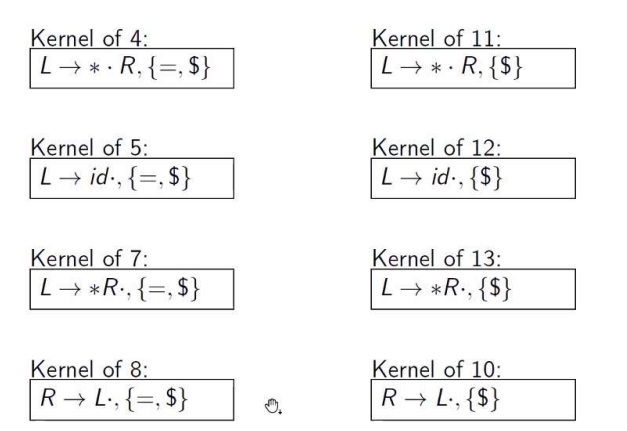
\includegraphics[width=.8\textwidth]{send_help_7.png}
    \caption{help}
\end{figure}
SI nota di fatto che tra i due automi lr0 e lr1 esiste una sottostruttura che è replicata in entrambi,
questa similarità si presenta esattamente in questi stati.
Il processo verso l'automa lalr prevede di passare per l'automa intermedio LRm(1), ovvero LR(1)
merged
Tutti gli stati di lr1 ma si mergiano quegli stati che appunto hanno lr0 item uguali tra di loro
Ad esempio lo stato 4 e lo stato 11 hanno esattamente gli stessi item-LR(0), quindi si possono
mergiare!
Gli stati dell'automa LRm1 sono:
Le transizioni invece:
\begin{figure}[H]
    \centering
    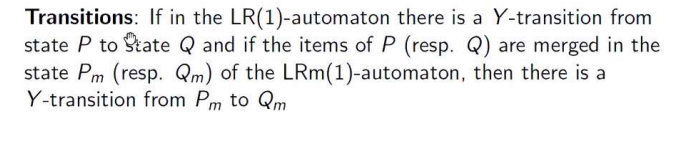
\includegraphics[width=.8\textwidth]{send_help_8.png}
    \caption{help}
\end{figure}
Ora che ho l'automa LRm(1) costruisco la tabella di parsing LALR in questo modo:

- Utilizzo l'automa LRm(1) per costruire la tabella
- Le riduzioni le decido utilizzando come lookahead function l'unione dei \(\Delta\) degli item-LR(1)
degli stati (se uno stato è merged vado a vedere tutti i singoli Delta degli stati che ho mergiato) - Ora che ho l'automa LRm(1) costruisco la tabella di parsing LALR in questo modo:

%IN QUALCHE MODO STE PARTI SI DEVONO COLLEGARE IDKH

\subsubsection{Caso di studio parsing LR(1)}

Prendiamo ancora una volta in considerazione la seguente grammatica:
\begin{align*}
    S &\to L = R \mid R \\
    L &\to *R \mid id \\
    R &\to L
\end{align*}

Costruendo l'automa caratteristico sia per il parsing di tipo SLR(1) sia LR(1) abbiamo affermato che non si trattasse di una di una grammatica SLR(1), in quanto conteneva dei conflitti, bensì di una LR(1).

Nel caso SLR(1) infatti gli item di riduzione vengono trasformati in operazioni di reduce in presenza dei follow del driver delle produzioni. 

Lo stato che genera un conflitto all'interno del automa caratteristico SLR(1) è quello identificato dal numero 2: utilizzando come detto precedentemente i follow non riusciamo ad avere un'espressività tale da discriminare le operazioni di reduce e di shift che vanno a creare un s/r conflict; utilizzando un parsing LR(1) nel medesimo stato avremo invece un'operazione di \texttt{shift 6} solo nel caso in cui leggessimo \{=\} dall'input buffer mentre invece \texttt{reduce \(R \to L\)} nel caso in cui il simbolo letto in input sia \{\$\}.

Supponiamo a questo proposito di fare un'analisi di una stringa del tipo \(w_1 = w_2\) utilizzando l'automa caratteristico LR(1): visto che l'uguale è un simbolo generato solo se si sceglie una produzione del tipo \(S \to L = R\), una volta che abbiamo letto tutto ciò che fa a capo \(w_1\) dobbiamo fare una riduzione ad \(L\).

A questo punto però, osservando la grammatica, dovrebbe essere abbastanza chiaro che le uniche parole derivabili da \(L\) appartengono a \(\{*^n id \mid n \geq 0\}\) e che le uniche derivazioni di parole in \(\{*^n id \mid n > 0\}\) coinvolgono la \(R\) (i.e. se vogliamo una stringa in cui compaia almeno una volta il simbolo * è necessario utilizzare la produzione \(L \rightarrow *R\)).

Se la stringa che si sta analizzando è del tipo \(id = w_2\) allora ci spostiamo dallo stato 5 per poi effettuare \texttt{reduce \(L \to id\)} e spostarci allo stato 2. 

Se invece ci stiamo concentrando su una stringa del tipo \(*w_1' = w_2\) allora ci sposteremo invece allo stato 4 dove continueremo a eseguire un ciclo fino a che non esauriremo gli \(*\): nel momento in cui leggeremo invece \(id\) ci sposteremo allo stato 5, eseguiremo \texttt{reduce \(L \to id\)} e finiremo con lo spostarci allo stato 8 e \textbf{non} al 2. 

Il parsing di tipo SLR(1) non riconosce dunque la differenza fra lo stato 2 e lo stato 8 a differenza del parsing LR(1) che ha un costo maggiore. 

Il problema nel caso del parsing SLR(1) è che andiamo a piazzare un'operazione di reduce per tutti i follow dei driver mentre in quello di tipo LR(1) lo si fa per sottoinsiemi dei follow dei driver.

\section{Parsing LRm(1)}

Nonostante il parsing di tipo LR(1) sia il più completo è possibile che l'automa caratteristico risultante contenga delle ridondanze: nell'esempio precedente vi sono infatti delle sottostrutture che sono isomorfe e ciò deriva dal fatto che, visto che le transizioni dipendono sempre dalla prima componente (i.e. item LR(0)), è possibile notare che le ridondanze si verificano nel caso in cui gli stati abbiano la stessa proiezione LR(0).

\subsection{Automi LRm(1)}

L'automa LRm(1) \(\mathcal{AM}\) è costruito a partire dall'automa LR(1) \(\mathcal{A}\) (la lettera m sta per \emph{merged}).

Gli \textbf{Stati} del nuovo automa caratteristico sono ottenuti unendo all'interno di un singolo stato di \(\mathcal{AM}\) tutti gli item negli stati \(<P_1, ..., P_n>\) di \(\mathcal{A}\) che hanno le stesse LR(0)-proiezioni (i.e. con lo stesso item LR(0)).

\textbf{Transizioni}: Se lo stato \(P\) di \(\mathcal{A}\) ha la stessa \(Y\)-transizione a \(Q\) e se \(P\) è stato unito in \(<P_1, ..., P_n>\) e \(Q\) in \(<Q_1, ..., Q_m>\), allora c'è una \(Y\)-transizione in \(\mathcal{AM}\) da \(<P_1, ..., P_n>\) a \(<Q_1, ..., Q_m>\).

Se prendiamo in considerazione l'automa LR(1) definito precedente, possiamo osservare che gli stati 4 e 11 hanno la medesima prima proiezione e quindi possiamo unirli all'interno di un nuovo stato.

Cosa facciamo per le transizioni? Nell'automa LR(1) abbiamo un'unica transizione etichettata \(id\) che va dallo stato 4 allo stato 5 (e allo stesso modo un'altra etichettata \(id\) dallo stato 11 al 12). Visto che gli stati 4 e 11 sono stati uniti in un unico stato (4\&11) e lo stesso vale per 5 e 12 (5\&12), per la definizione precedente possiamo inserire in \(\mathcal{AM}\) una transizione da 4\&11 a 5\&12 etichettata \(id\).

Eseguendo l'operazione descritta la dimensione (i.e. il numero di stati) dell'automa LRm(1) così generato è sicuramente uguale a quella dell'automa LR(0): andando a combinare stati con con gli stessi item LR(0) ci ritroveremo con lo stesso numero di stati dell'automa LR(0) e con lo stesse transizioni. 

\section{Parsing Table LALR(1)}

Le parsing table LALR(1) sono ottenute prendendo:

\begin{itemize}
    \item l'automa caratteristico LRm(1)
    \item la lookahead function \(\mathcal{LA}(P, A \to \beta) = \cup_{[A \to \beta \cdot, \Delta_j]} \Delta_j\)
\end{itemize}

Nel caso in cui non vi sia più di uno stato con la stessa proiezione LR(0) allora tale stato non subisce l'operazione di unione e viene inserito direttamente nell'automa LRm(1) con il medesimo lookahead-set.

La grammatica \(\G\) è LALR(1) se e solo se la sua tabella di parsing LALR(1) non ha conflitti. 

Il vantaggio della grammatica LALR(1) è di essere più potente (i.e. espressiva) della grammatica SLR(1) pur rimanendo con delle dimensioni contenute rispetto alla LR(1). 

\subsection{Esercizio parsing LALR(1) - c'è sì ma in realtà no perchè è LR(1)}
\begin{align*}
    S &\to AaB \mid b \\
    A &\to BcBaA \mid \epsilon \\
    B &\to \epsilon
\end{align*}

Il nostro obbiettivo è quello di costruire la parsing table LALR(1) per la grammatica citata: per poter procedere dobbiamo però prima costruire l'automa caratteristico.
\paragraph{Ricaviamo l'automa}
\begin{enumerate}
    \item Inizializziamo lo stato 0; il suo kernel è 
    \begin{equation*}
        S' \to \cdot S, \{\$\}
    \end{equation*}
    Di questo kernel devo calcolare la chiusura:
    \begin{align*}
        S &\to \cdot AaB, \{\$\} \\
        S &\to \cdot b, \{\$\} \\
        A &\to \cdot BcBaA, \{a\} \\
        A &\to \cdot, \{a\} \\
        B &\to \cdot, \{c\}
    \end{align*}
    Essendo questi gli item per lo stato 0, possiamo identificare quattro possibili transizioni (e quindi quattro possibili nuovi stati): \(\tau(0,S)=1 \textrm{, } \tau(0,A)=2 \textrm{, } \tau(0,b)=3 \textrm{ e } \tau(0,B)=4\).
    
    Interessante notare che le produzioni del tipo \(A \to \epsilon\) vengono convertite in reducing item \(A \to \cdot\).
    \item Analizziamo ora lo stato 1; il suo kernel è 
    \begin{equation*}
        S' \to S \cdot, \{\$\}    
    \end{equation*}
    Non serve calcolare la chiusura di questo item in quanto è formata solamente da sé stesso, possiamo però evidenziare il fatto che questo è lo stato contenente l'\textbf{Accepting Item}.
    \item Analizziamo dunque lo stato 2, il cui kernel è composto solamente da:
    \begin{equation*}
        S \to  A \cdot aB, \{\$\}
    \end{equation*}
    Nemmeno in questo caso è necessario calcolare la sua chiusura in quanto il marker si trova davanti ad un non terminale: aggiungiamo dunque la transizione \(\tau(2,a)=5 \) e proseguiamo.
    \item Il kernel dello stato 3 è dato da
    \begin{equation*}
        S \to b \cdot, \{\$\}
    \end{equation*}
    Il che vuol dire che non è possibile calcolare la chiusura e che lo stato 3 contiene un reducing item.
    \item Passiamo allo stato 4, il cui kernel è:
    \begin{equation*}
        A \to B \cdot cBaA, \{a\} 
    \end{equation*}
   Per gli stessi motivi dello stato 2 la chiusura di tale stato non porta nuovi elementi; è comunque possibile definire la transizione \(\tau(4,c)\) allo stato 6
    \item Il kernel dello stato 5 è:
    \begin{equation*}
        S \to  Aa \cdot B, \{\$\}
    \end{equation*}
    La cui chiusura risulta essere pari a 
    \begin{align*}
        B &\to \cdot, \{\$\}
    \end{align*}
    Per questo motivo sappiamo che lo stato contiene un reducing item e possiede una transizione \(\tau(5, B)\) allo stato 7
    \item Procedendo come abbiamo fatto fino ad ora il kernel per lo stato 6 è
    \begin{equation*}
        A \to Bc \cdot BaA, \{a\} 
    \end{equation*}
    la cui chiusura corrisponde a 
    \begin{equation*}
         B \to \cdot, \{a\} 
    \end{equation*}
    Come è intuibile lo stato 6 contiene un reducing item e la sua transizione è \(\tau(6, B)=8\)
    \item Il kernel dello stato 7 è 
    \begin{equation*}
         S \to  AaB \cdot, \{\$\}  
    \end{equation*}
    Essendo che il marker è in fondo alla produzione non è possibile effettuare la chiusura ma solo considerare che lo stato 7 contiene un reducing item
    \item Lo stato 8 ha kernel
    \begin{equation*}
        A \to BcB \cdot aA, \{a\} 
    \end{equation*}
    e possiede una transizione \(\tau(8, a)\) allo stato 9
    \item Lo stato 9 ha kernel
    \begin{equation*}
        A \to BcBa \cdot A, \{a\} 
    \end{equation*}
    di cui possiamo computare la chiusura ottenendo
    \begin{align*}
        A &\to \cdot BcBaA, \{a\} \\
        A &\to \cdot, \{a\} \\
        B &\to \cdot, \{c\}
    \end{align*}
    Che contiene due reducing item e possiede due transizioni: la prima è \(\tau(9, A)=10\) e ha come target un nuovo stato mentre la seconda è \(\tau(9, B)=4\) che ha come target uno stato che fa già parte del nostro automa caratteristico.
    \item Lo stato 10 infine ha kernel
    \begin{equation*}
        A \to BcBaA \cdot, \{a\} 
    \end{equation*}
    Visto che il marker è posto alla fine non è possibile calcolare la chiusura di questo stato e possiamo concludere aggiungendo che lo stato 10 ha un reducing item. 
\end{enumerate}

L'automa caratteristico LR(1) risulta dunque così costruito

\begin{figure}[H]
	\centering
	\subimport{assets/figures/}{automa_LR-LALR.tex}
    \caption{Automa LR(1)/LALR(1)}
    \label{fig:lalr-automata}
\end{figure}

Visto che non è possibile unire nessuno degli stati dell'automa LR(1), l'automa disegnato poc'anzi corrisponderà anche a quello LRm(1). Di seguito dunque possiamo costruire la tabella di parsing

\begin{enumerate}
    \item \(S \to AaB\) 
    \item \(S \to b\) 
    \item \(A \to BcBaA\) 
    \item \(A \to \epsilon\) 
    \item \(B \to \epsilon\)
\end{enumerate}

\begin{table}[h]
    \centering
    \subimport{assets/tables/}{lr-lalr-parsing-table.tex}
    \caption{LR(1) \& LALR(1) Parsing Table}
    \label{tab:lr-lalr-parsing-table}
\end{table}


\section{Calcolo dell'LRm(1) automa tramite l'automa simbolico}
La classe di grammatiche LALR contiene le grammatiche più interessanti per i linguaggi di programmazione.
Abbiamo visto come la modalità più semplice per ottenere le tabelle di parsing LALR è quella di creare in primis un'automa LR(1) e poi tradurlo in LRm(1).

Oggi vediamo un altro metodo che prevede di eliminare il passaggio dall'automa LR(1) e di creare fin da subito un automa con la stessa struttura dell'automa LRm(1).
Quello che andremo a creare è detto automa simbolico, preché utilizza dei simboli (delle variabili) al posto dei lookahead set; una votla terminata la costruzione dell'automa simbolico risolvendo i simboli si va a calcolare quelli che poi saranno i lookahead set dell'automa LRm(1).

Quindi gli item di questo automa simbolico possono essere immaginati cme suddivisi in due componenti:
\begin{itemize}
    \item una componente di tipo LR(0);
    \item una parte composta da un insieme di lookahead simbolico.
\end{itemize}
Sostanzialmente questi item sono del tutto assimilabili agli item LR(1), con l'unica differenza che il \(\Delta\) set è simbolico e presto al lettore sarà ben chiaro questo concetto.

Mentre creaimo l'automa simbolico ci memorizziamo in una tabella delle equazioni che ci serviranno alla fine per tradurre i lookahead set simbolici in lookahead effettivi. Come è ormai consuetudine il modo più semplice per spiegare questo procedimento è applicarlo direttamente ad un esempio.

\subsection{Esempio di costruzione dell'automa simbolico}
Andiamo a costruire l'automa simbolico per la nostra cara grammatica
\begin{align*}
    S &\to L = R \mid R \\
    L &\to *R \mid id \\
    R &\to L
\end{align*}
La costruzione dell'automa simbolico verrà affiancata dalla costruzione dell'automa LR(1) per rendere più chiare le differenze tra queste due costruzioni.

Il primo passo è installare lo stato 0 dell'automa:
\begin{figure}
    \centering
    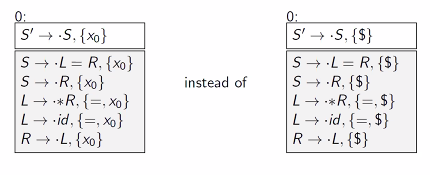
\includegraphics[width=.7\textwidth]{ex_automa_simbolico-stato_0.png}
    \caption{Stato 0: sulla sinistra automa simbolico, sulla destra automa LR(1)}
    \label{img:ex_automa_simbolico-stato_0}
\end{figure}
È subito chiaro cosa intendevamo dicendo "invece di inserire il lookahead set inseriamo una \emph{variabile}", di fatto come lookahead inseriamo un simbolo, che risolveremo solo alla fine della costruzione dell'automa.

In questo caso al posto di inserire \(\$\) inseriamo una variabile chiamata \(x_0\).
La corrispondenza tra \(x_0\) e \(\$\) la salviamo (ce la scriviamo) nel sitema di equazioni che ci porteremo dietro per tutta la costruzione.
\begin{align*}
    Sistema:& \\
            & x_0 = \{\$\}
\end{align*}

Quando andiamo a fare la chiusura, essendo gli item simbolici in tutto e per tutto simili agli item LR(1), utilizziamo la \(closure_1\).
Questa volta però abbiamo come lookahead set le variabili, in questo caso il nostro lookahead set è \(x_0\).

Procedendo un passettino alla volta la chiusura dello stato 0 si fa così:
\begin{itemize}
    \item in primis dobbiamo includere la chiusura per le produzioni di S:
    \begin{itemize}
        \item dalle due prduzioni di \(S\) della nostra grammatica otteniamo i due item:
        \begin{align*}
            S &\to \cdot L = R,  \; \{x_0\} \\
            S &\to \cdot R,  \; \{x_0\}
        \end{align*}
        in questo caso il lookahead set è facile da calcolare perché \(\beta = \varepsilon\) mentre \(\Delta = x_0\);
    \end{itemize}
    \item ora abbiamo introdotto anche un marker davanti alla \(L\), quindi dobbiamo chiudere anche per \(L\):
    \begin{itemize}
        \item dalle produzioni di \(L\) otteniamo i due item:
        \begin{align*}
            L &\to \cdot *R, \; \{=\} \\
            L &\to \cdot id, \; \{=\}
        \end{align*}
        in questo caso, dato che \(\beta \neq \epsilon\), vediamo come il lookahead set corrisponda ad un carattere e non una variabile, questo è possibile mentre stiamo calcolando la chiusura di item simbolici;
    \end{itemize}
    \item infine, avendo introdotto anche \(R\), dobbiamo calcolare la chiusura indotta dalle produzioni di \(R\):
    \begin{itemize}
        \item abbiamo solo una produzione per \(R\), che ci porta ad inserire l'item 
        \begin{equation*}
            R \to \cdot L, \; \{x_0\}
        \end{equation*}
        è andato tutto liscio come l'olio no?
    \end{itemize}
    \item invece no! perché abbiamo introdotto una nuova chiusura per \(L\), che è diversa dalla precedente perché ora il lookahead set della chiusura è \(x_0\) invece che \(=\), quindi quello che dobbiamo fare è ricalcolare le chiusure di \(L\) con questo nuovo lookahead; dato che siamo skillati e sappiamo già come andrà a finire aggiungiamo semplicemente \(\{x_0\}\) al lookahead set delle produzioni di \(L\) che abbiamo già elencato poco fa, quindi:
    \begin{align*}
        L &\to \cdot *R, \; \{=, x_0\} \\
        L &\to \cdot id, \; \{=, x_0\}
    \end{align*}
\end{itemize}
Il consiglio per chi non ha capito questi passaggi è quello di fare qualche esercizio di costruzione di automi LR(1), fidatevi ne vale la pena!

Orbene, passiamo ad analizzare le transazioni uscenti dallo stato 0.
La prima transizione che troviamo è \(\tau(0,S)\) che ci porta ad un nuovo stato, lo stato 1.
\\
Kernel dello stato 1:
\begin{figure}
    \centering
    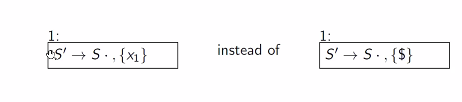
\includegraphics[width=.7\textwidth]{ex_automa_simbolic-kernel_s1.png}
    \caption{Kernel stato 1: sulla sinistra automa simbolico, sulla destra automa LR(1)}
\end{figure}
notiamo come invece che scrivere il lookahead set come insieme creiamo una nuova variabile per indicarlo. Dobbiamo aggiornare anche il nostro sitema in cui salviamo il valore effettivo della variabile.
In questo caso il lookahed set del kernel, essendo \(\beta = \varepsilon\) è proprio uguale al lookahead set della produzione da cui arriviamo, quindi \(x_0\), aggiorniamo dunque alacremente il nostro sistema di equazioni.
\begin{align*}
    Sistema:& \\
            & x_0 = \{\$\} \\
            & x_1 = x_0
\end{align*}
Lo stato 1 non ha chiusure da calcolare e nemmeno transizioni, quindi passiamo oltre.

La prossima transizione che andiamo ad analizzare è \(\tau(0,L)\) che ci porta in un nuovo stato, diciamo 2.
\\
Kernel dello stato 2:
\begin{figure}
    \centering
    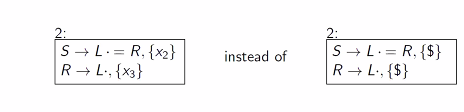
\includegraphics[width=.7\textwidth]{ex_automa_simbolico-kernel_s2.png}
    \caption{Kernel stato 2: sulla sinistra automa simbolico, sulla destra automa LR(1)}
\end{figure}
in questo caso il kernel contiene due item perché nello stato 0 abbiamo due item che presentano la possibilità di una \(L\)-transizione; ognuno di questi item quindi avrà il suo lookahead set simbolico: andiamo ad aggiornare subito il nostro sistema, sapendo che le produzioni che ci portano allo stato due hanno come lookahead set \(x_0\).
\begin{align*}
    Sistema:& \\
            & x_0 = \{\$\} \\
            & x_1 = x_0 \\
            & x_2 = x_0 \\
            & x_3 = x_0 \\
\end{align*}
grazie al cielo non si presentano nè chiusure, le transizioni invece le analizzeremo in seguito.

Passiamo quindi all'osservazione della transizione \(\tau(0,R)\), che ci porta nello stato 3.
\\
Kernel dello stato 3:
\begin{figure}
    \centering
    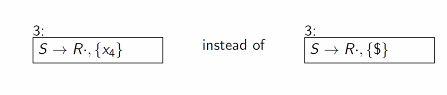
\includegraphics[width=.7\textwidth]{ex_automa_simbolico-kernel_s3.png}
    \caption{Kernel stato 3: sulla sinistra automa simbolico, sulla destra automa LR(1)}
\end{figure}
anche in questo caso abbiamo che \(\beta = \varepsilon\) quindi il lookahead set del kernel è uguale a \(\Delta\), riportiamo subito questa informazione all'interno del sistema.
\begin{align*}
    Sistema:& \\
            & x_0 = \{\$\} \\
            & x_1 = x_0 \\
            & x_2 = x_0 \\
            & x_3 = x_0 \\
            & x_4 = x_0 \\
\end{align*}
il kernel dello stato 3 non presenta nè chiusure nè transizioni, quindi procediamo oltre senza esitazioni.

La prossima transizione che dobbiamo analizzare è \(\tau(0,*)\), questa deriva dalla produzione \([L \to \cdot *R, \; \{=, x_0\}]\).
\\
Kernel dello stato 4:
\begin{figure}
    \centering
    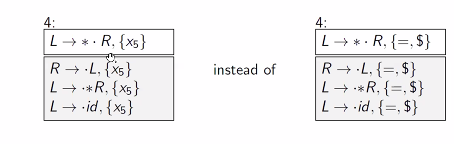
\includegraphics[width=.7\textwidth]{ex_automa_simbolico-kernel_s4.png}
    \caption{Kernel stato 4: sulla sinistra automa simbolico, sulla destra automa LR(1)}
\end{figure}
anche in questo caso  \(\beta = \varepsilon\) quindi il lookahead set del kernel è uguale a \(\Delta\), aggiorno quindi il sistema di equazioni.
\begin{align*}
    Sistema:& \\
            & x_0 = \{\$\} \\
            & x_1 = x_0 \\
            & x_2 = x_0 \\
            & x_3 = x_0 \\
            & x_4 = x_0 \\
            & x_5 = \{=, \$\}
\end{align*}
finalmente uno stato che ci dia la \emph{soddisfazione} di calcolare delle chiusure, grazie alle produzioni di \(R\) in primis e di \(L\) poi otteniamo la seguente chiusura per gli item dello stato 4:
\begin{align*}
    R &\to \cdot L, \; \{x_5\} \\
    L &\to \cdot *R, \; \{x_5\} \\
    L &\to \cdot id, \; \{x_5\}
\end{align*}
che spettacolo, eh? passiamo oltre

Prossima transizione da analizzare: \(\tau(0,id)\) che deriva dall'item \([L \to \cdot id, \; \{=, x_0\}]\) e ci porta nello stato 5.
\\
Kernel dello stato 5:
\begin{figure}
    \centering
    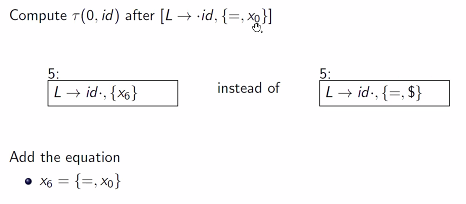
\includegraphics[width=.7\textwidth]{ex_automa_simbolico-kernel_s5.png}
    \caption{Kernel stato 5: sulla sinistra automa simbolico, sulla destra automa LR(1)}
\end{figure}
anche in questo caso  \(\beta = \varepsilon\) quindi il lookahead set del kernel è uguale a \(\Delta\), aggiorno quindi il sistema di equazioni.
\begin{align*}
    Sistema:& \\
            & x_0 = \{\$\} \\
            & x_1 = x_0 \\
            & x_2 = x_0 \\
            & x_3 = x_0 \\
            & x_4 = x_0 \\
            & x_5 = \{=, \$\} \\
            & x_6 = \{=, \$\} \\
\end{align*}
Anche qui, pace all'anima nostra, inseriamo il lookahead set come variabile e la valorizziamo nel nostro sistema di equazioni.

Abbiamo finito le transizioni dallo stato 0! prossima trnsizione da analizzare \(\tau(2, =)\), che deriva dall'item \([S \to L \cdot = R, \; \{x_2\}]\), ci porta direttamente allo stato 6.
\\
Kernel dello stato 6:
\begin{figure}
    \centering
    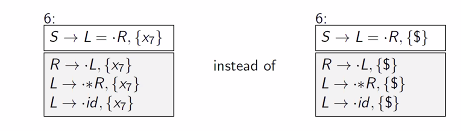
\includegraphics[width=.7\textwidth]{ex_automa_simbolico-kernel_s6.png}
    \caption{Kernel stato 6: sulla sinistra automa simbolico, sulla destra automa LR(1)}
\end{figure}
in questo caso  \(\beta = \varepsilon\) quindi il lookahead set del kernel è uguale a \(\Delta\), aggiorno quindi il sistema di equazioni.
\begin{align*}
    Sistema:& \\
            & x_0 = \{\$\} \\
            & x_1 = x_0 \\
            & x_2 = x_0 \\
            & x_3 = x_0 \\
            & x_4 = x_0 \\
            & x_5 = \{=, \$\} \\
            & x_6 = \{=, \$\} \\
            & x_7 = x_2 \\
\end{align*}
Ora passiamo ad analizzare le chiusure degli item di questo stato.
Grazie alla presenza del marker davanti ad una \(R\) aggiungiamo questi item allo stato:
\begin{align*}
    R &\to \cdot L, \; \{x_7\} \\
    L &\to \cdot *R, \; \{x_7\} \\
    L &\to \cdot id, \; \{x_7\}
\end{align*}

Passiamo ora ad analizzare la transizione \(\tau(4, R)\), che deriva dall'item \([L \to * \cdot R, \; \{x_5\}]\) e ci spara nello stato 7.
\\
Kernel dello stato 7:
\begin{figure}
    \centering
    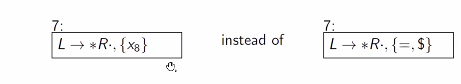
\includegraphics[width=.7\textwidth]{ex_automa_simbolico-kernel_s7.png}
    \caption{Kernel stato 7: sulla sinistra automa simbolico, sulla destra automa LR(1)}
\end{figure}
in questo caso  \(\beta = \varepsilon\) quindi il lookahead set del kernel è uguale a \(\Delta\), aggiorno quindi il sistema di equazioni.
\begin{align*}
    Sistema:& \\
            & x_0 = \{\$\} \\
            & x_1 = x_0 \\
            & x_2 = x_0 \\
            & x_3 = x_0 \\
            & x_4 = x_0 \\
            & x_5 = \{=, \$\} \\
            & x_6 = \{=, \$\} \\
            & x_7 = x_2 \\
            & x_8 = x_5 \\
\end{align*}
a questo punto dovremmo fare la chiusura no? ma è già tutto chiuso, come alle 23:30 di sera a Trento...

Passiamo quindi ad analizzare la transizione \(\tau(4, L)\) che prende le mosse dall'item \([R \to \cdot L, \; \{x_5\}]\) e ci porta nello stato 8.
\\
Kernel dello stato 8:
\begin{figure}
    \centering
    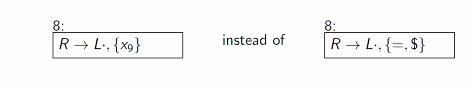
\includegraphics[width=.7\textwidth]{ex_automa_simbolico-kernel_s8.png}
    \caption{Kernel stato 8: sulla sinistra automa simbolico, sulla destra automa LR(1)}
\end{figure}
in questo caso il lookahead set del kernel è uguale a \(\Delta\), aggiorno quindi il sistema di equazioni.
\begin{align*}
    Sistema:& \\
            & x_0 = \{\$\} \\
            & x_1 = x_0 \\
            & x_2 = x_0 \\
            & x_3 = x_0 \\
            & x_4 = x_0 \\
            & x_5 = \{=, \$\} \\
            & x_6 = \{=, \$\} \\
            & x_7 = x_2 \\
            & x_8 = x_5 \\
            & x_9 = x_5 \\
\end{align*}
anche qui niente chiusure.

Passiamo ad analizzare la transizione \(\tau(4,*)\), che deriva dall'item \([L \to \cdot * R, \{x_5\}]\); ora, se osserviamo bene il kernel dello stato in cui arriveremmo tramite questa transizione ci rediamo conto che è un kernel che abbiamo già incontrato, nello specifico proprio nello stato 4 da cui stiamo partendo, cosa significa tutto ciò?

Significa semplicemente che c'è un arco uscente da 4 che ci riporta in 4 (self loop in gergo) tramite una \(*\)-transizione. È qui che vediamo finalmente la grande differenza di costruzione tra automi LR(1) ed automi simbolici: in un automa LR(1) avremmo costruito un nuovo stato (perché il lookahead set in questo caso è diverso dal lookahead set dello stato 4), invece ora andiamo semplicemente ad aggiornare il lookahead set dello stato 4 con il lookahead set della transizione  \(\tau(4,*)\) (che fatalità corrisponde propiro a \(x_5\)).
\begin{align*}
    Sistema:& \\
            & x_0 = \{\$\} \\
            & x_1 = x_0 \\
            & x_2 = x_0 \\
            & x_3 = x_0 \\
            & x_4 = x_0 \\
            & x_5 = \{=, \$\} \cup \{x_5\} \\
            & x_6 = \{=, \$\} \\
            & x_7 = x_2 \\
            & x_8 = x_5 \\
            & x_9 = x_5 \\
\end{align*}

Passiamo ora ad analizzare la transizione \(\tau(4, id)\), che deriva dall'item \([L \to \cdot id, \; \{x_5\}]\), colpo di scena! anche questo kernel ci è noto, corrisponde a quello dello stato 5, quindi andiamo ad aggiornare il lookahead set dello stato 5.
Il lookahead set della transizione \(\tau(4, id)\) è ancora una volta \(x_5\).
\begin{align*}
    Sistema:& \\
            & x_0 = \{\$\} \\
            & x_1 = x_0 \\
            & x_2 = x_0 \\
            & x_3 = x_0 \\
            & x_4 = x_0 \\
            & x_5 = \{=, \$\} \cup \{x_5\} \\
            & x_6 = \{=, \$\} \cup \{x_5\} \\
            & x_7 = x_2 \\
            & x_8 = x_5 \\
            & x_9 = x_5 \\
\end{align*}

Passiamo oltre, la prossima transizione su cui ci concentriamo è \(\tau(6, R)\), derivante da \([S \to L = \cdot R, \; \{x_7\}]\), che ci porta a scoprire lo stato 9.
\\
Kernel dello stato 9:
\begin{figure}
    \centering
    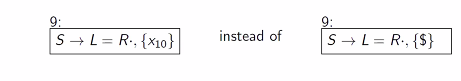
\includegraphics[width=.7\textwidth]{ex_automa_simbolico-kernel_s9.png}
    \caption{Kernel stato 9: sulla sinistra automa simbolico, sulla destra automa LR(1)}
\end{figure}
in questo caso  \(\beta = \varepsilon\) quindi il lookahead set del kernel è uguale a \(\Delta\), ovvero \(x_{10} = \{x_7\}\), aggiorno quindi il sistema di equazioni.
\begin{align*}
    Sistema:& \\
            & x_0 = \{\$\} \\
            & x_1 = x_0 \\
            & x_2 = x_0 \\
            & x_3 = x_0 \\
            & x_4 = x_0 \\
            & x_5 = \{=, \$\} \cup \{x_5\} \\
            & x_6 = \{=, \$\} \cup \{x_5\} \\
            & x_7 = x_2 \\
            & x_8 = x_5 \\
            & x_9 = x_5 \\
            & x_{10} = x_7 \\
\end{align*}
anche questo kernel ci regala poche emozioni (e nessuna chiusura) quindi concludiamo l'analisi dello stato 9.

La prossima transizione è \(\tau(6, L)\) che deriva da \([R \to \cdot L, \{x_7\}]\); tale transizione ci porterebbe in uno stato con kernel LR(0) = \([R \to L \cdot ]\), che quindi corrisponde al nostro stato 8: invece che creare un nuovo stato andiamo ad aggiornare il lookahead set dello stato 8 con il lookahead set che deriva dalla transizione \(\tau(6, L)\).
\begin{align*}
    Sistema:& \\
            & x_0 = \{\$\} \\
            & x_1 = x_0 \\
            & x_2 = x_0 \\
            & x_3 = x_0 \\
            & x_4 = x_0 \\
            & x_5 = \{=, \$\} \cup \{x_5\} \\
            & x_6 = \{=, \$\} \cup \{x_5\} \\
            & x_7 = x_2 \\
            & x_8 = x_5 \\
            & x_9 = x_5 \cup \{x_7\} \\
            & x_{10} = x_7 \\
\end{align*}
niente chiusure, passiamo oltre.

Prossima transizione \(\tau(6, *)\), derivante dall'item \([L \to \cdot * R, \{x_7\}]\), il target di questa transizione è uno stato con kernel LR(0) \([L \to *\cdot R]\), ovvero lo stato 4. Quindi anche questa volta non creiamo un nuovo stato ma andiamo ad aggionrare il kernel dello stato 4.
\begin{align*}
    Sistema:& \\
            & x_0 = \{\$\} \\
            & x_1 = x_0 \\
            & x_2 = x_0 \\
            & x_3 = x_0 \\
            & x_4 = x_0 \\
            & x_5 = \{=, \$\} \cup \{x_5\} \cup \{x_7\} \\
            & x_6 = \{=, \$\} \cup \{x_5\} \\
            & x_7 = x_2 \\
            & x_8 = x_5 \\
            & x_9 = x_5 \cup \{x_7\} \\
            & x_{10} = x_7 \\
\end{align*}

Passiamo alla prossima transizione che è \(\tau(6, id)\), derivante da \([L \to \cdot id, \{x_7\}]\), che ci porta in uno stato con kernel LR(0) = \([L \to id \cdot]\), che corrisponde al già visitato stato 5, quindi aggiorniamo semplicemente il lookahead set di tale stato.
\begin{align*}
    Sistema:& \\
            & x_0 = \{\$\} \\
            & x_1 = x_0 \\
            & x_2 = x_0 \\
            & x_3 = x_0 \\
            & x_4 = x_0 \\
            & x_5 = \{=, \$\} \cup \{x_5\} \cup \{x_7\} \\
            & x_6 = \{=, \$\} \cup \{x_5\} \cup \{x_7\} \\
            & x_7 = x_2 \\
            & x_8 = x_5 \\
            & x_9 = x_5 \cup \{x_7\} \\
            & x_{10} = x_7 \\
\end{align*}

Oh butei, abbiamo finito di analizzare l'automa, quindi andiamo a risolvere lo strascico di equazioni che ci siamo tirati dietro per tutto l'esercizio:
\begin{align*}
    x_0, x_1, x_2, x_3, x_4, x_7, x_{10} &= \{\$\} \\
    x_5, x_6, x_8, x_9 &= \{=, \$\}
\end{align*}
Questa risoluzione è fatta a occhio, ma esiste un metodo algoritmico per risolvere il sistema in modo molto efficiente.
L'algoritmo in questione utilizzale classi di equivalenza, inaspettatamente.

Complessivamente cosa abbiamo ottenuto?
Un automa con le stesse dimensioni di tipo LR(0), poichè abbiamo creato esattamente gli stessi stati che avremmo cerato costruendo un automa LR(0), ma abbiamo utilizzato delle chiusure di tipo LR(1), ricavando quindi dei lookahead set raffinati.

Per concludere questo esempio ricordiamo brevemente quali sarebbero i passi da seguire a questo punto per ottenere l'automa merged:
\begin{enumerate}
    \item inseriamo tutti gli stati;
    \item le mosse di shift (le transizioni) sono sesattamente quelle identificate e corrispondono alle transizioni dell'automa caratteristico LR(0) per questa grammatica;
    \item gli stati con riduzioni sono tutti quelli che presentatno una produzione con il marker in fondo al body;
    \item le lookahead function (le etichette per le riduizioni) corrispondono ai lookahead set calcolati nella risoluzione del sistema.
\end{enumerate}
Carino questo esempio, eh? per festeggiare il suo completamento ci concediamo la risoluzione di un altro esercizio dello stesso tipo.

\subsection{Esercizio di costruzione dell'automa simbolico}
La grammatica di cui vogliamo ricavare l'automa simbolico questa volta è la nostra cara
\begin{equation}
    S \to aSb \mid ab
\end{equation}
Empezamos con lo stato 0.
\\
Kernel dello stato 0:
\begin{align*}
    S' \to \cdot S, x_0
\end{align*}
Ci salviamo il valore di \(x_0\).
\begin{align*}
    Sistema:& \\
            & x_0 = \{\$\}
\end{align*} 
Passiamo alla chiusura del kernel:
\begin{align*}
    S &\to \cdot aSb, x_0 \\
    S &\to \cdot ab, x_0
\end{align*}
Lo stato 0 non ci regala altre chiusure, ma ci regala due belle transizioni, una per \(a\) ed una per \(S\).
\\\\
Analizziamo quindi la transizione \(\tau(0,S)\), che ci porta nel nuovo stato 1.
\\
Kernel dello stato 1:
\begin{align*}
    S' \to S \cdot, x_1
\end{align*}
In questo caso \(\beta = \varepsilon\), quindi il lookahead set del kernel sarà ugualeal lookahead set della produaizone che ci ha portati in 1, ci salviamo questo risultato.
\begin{align*}
    Sistema:& \\
            & x_0 = \{\$\}\\
            & x_1 = x_0
\end{align*}
Questo stato non ci offre altri divertimenti, passiamo oltre.
\\\\
Analizziamo la transizione \(\tau(0,a)\), che ci porta nel nuovo stato 2.
\\
Kernel dello stato 2:
\begin{align*}
    S &\to  a \cdot S b, x_2 \\
    S &\to  a \cdot b, x_3
\end{align*}
In questo caso il lookahead set di entrambe le produzioni del kernel sarà uguale al lookahead della produzione che ci ha portato in 2, poiché \(\beta = \varepsilon\) in entrambi i casi.
\begin{align*}
    Sistema:& \\
            & x_0 = \{\$\}\\
            & x_1 = x_0 \\
            & x_2 = x_0 \\
            & x_3 = x_0
\end{align*}
In questo caso il primo item del kernel richiede che venga calcolata una chiusura:
\begin{align*}
    S &\to  \cdot a S b, \{b\} \\
    S &\to  \cdot a b, \{b\}
\end{align*}
Ma questa volta dobbiamo prestare attenzione perché la chiusura per \(S\) ha come \(\beta\) il carattere \(b\), quindi il lookahead set dei due item appena  ottenuti è \(\{b\}\).
Ora che abbiamo calcolato la chiusura del kernel possiamo passare alla prossima transizione.
\\\\
Analizziamo quindi \(\tau(2,S)\), che ci porta allo stato 3 tramite l'item \([S \to a \cdot S b, x_2]\).
\\
Kernel dello stato 3:
\begin{align*}
    S &\to  a S \cdot b, x_4
\end{align*}
Orbene, aggiorniamo il nostro sistema equatoriale sapendo che \(\beta = b\) mentre \(\Delta = x_2\).
\begin{align*}
    Sistema:& \\
            & x_0 = \{\$\}\\
            & x_1 = x_0 \\
            & x_2 = x_0 \\
            & x_3 = x_0 \\
            & x_4 = \{b\}
\end{align*}
Lo stato 3 non ci offre ulteriori motivi di svago.
\\\\
La prossima produzione che analizziamo è  \(\tau(2,b)\), che ci capitombola nel nuovo stato 4 tramite l'item \([S \to a \cdot b, \{x_3\}]\).
\\
Kernel dello stato 4:
\begin{align*}
    S \to  a b \cdot, x_5
\end{align*}
A questo punto devo aggiornare il sistema, tenendo conto che in questo caso non si applica la famosa forma \([A \to \alpha \cdot B \beta]\), quindi il lookahead set del kenrel di 4 sarà esattamente il lookahead set della produzione che ci ha portati in 4.
\begin{align*}
    Sistema:& \\
            & x_0 = \{\$\}\\
            & x_1 = x_0 \\
            & x_2 = x_0 \\
            & x_3 = x_0 \\
            & x_4 = \{b\} \\
            & x_5 = x_3 
\end{align*}
Lo stato è chiuso.
\\\\
Passiamo ora ad analizzare la transizione \(\tau(2,a)\) che, tramite gli item \([S \to  \cdot a S b, \{b\}]\) e \([S \to  \cdot a b, \{b\}]\), ci porta in un nuovo stato, lo stato 5.
\\
Kernel dello stato 5:
\begin{align*}
    S &\to a \cdot S b, x_6 \\
    S &\to a \cdot b, x_7
\end{align*}
Ma c'è un colpo di scena, perché noi abbiamo già visto questo kernel una volta: è esattamente il kernel dello stato 2!
Quindi la procedura ci richiede di aggiornare solo il lookahead set dello stato 2, senza generare un nuovo stato 5.
\begin{align*}
    Sistema:& \\
            & x_0 = \{\$\}\\
            & x_1 = x_0 \\
            & x_2 = x_0 \cup \{b\} \\
            & x_3 = x_0 \cup \{b\} \\
            & x_4 = \{b\} \\
            & x_5 = x_3
\end{align*}
\\\\
Ci resta da analizzare la transizione \(\tau(3,b)\) che tramite l'item \([S \to a S \cdot b, \{x_4\}]\) ci porta al nuovo (per davvero questa volta) stato 5.
\\
Kernel dello stato 5:
\begin{align*}
    S &\to a S b \cdot, x_6
\end{align*}
In questo caso il lookahead set del kernel rimane uguale a quello della transizione che ci ha portato in 5.
\begin{align*}
    Sistema:& \\
            & x_0 = \{\$\}\\
            & x_1 = x_0 \\
            & x_2 = x_0 \cup \{b\} \\
            & x_3 = x_0 \cup \{b\} \\
            & x_4 = \{b\} \\
            & x_5 = x_3 \\
            & x_6 = x_4
\end{align*}
Questo stato è chiuso, quindi terminiamo la sua analisi.

Avendo analizzato le transizioni non ci rimane altro da fare se non risolvere il sistema di equazioni per valorizzare le nostre \(x\).
\begin{align*}
    x_0 = x_1 &= \{\$\} \\
    x_2 = x_3 = x_5 &= \{\$, b\} \\
    x_4 = x_6 &= \{b\} 
\end{align*}
Andiamo quindi, per curiosità, ad analizzare gli stati in cui sono presenti le riduzioni ed a piazzarvi i lookahead set:
\begin{itemize}
    \item in 1 abbiamo la riduzione \(S' \to S \cdot, \; \{\$\}\);
    \item in 4 abbiamo \(S \to a b \cdot, \; \{\$, b\}\);
    \item in 5 abbiamo \(S \to aSb \cdot, \; \{b\}\).
\end{itemize}
Notimao quindi che non si presentano conflitti, quindi la grammatica è di tipo LALR.


\section{Algoritmo Shift/Reduce}
% \section{Un primo esempio di applicazione}
% \subsection{Mosse di shift e reduce}
% Andiamo a introdurre l'algoritmo che utilizzeremo per verificare se una certa parola appartenga o meno al linguaggio denotato da una certa grammatica, rappresentata dal suo automa caratteristico; questo è detto algoritmo di shift/reduce, dal nome delle due mosse che andremo a utilizzare. Come prima cosa, prendiamo familiriatà con le due pile che utilizzeremo nella procedura:
% \begin{itemize}
%     \item nella prima inseriamo gli stati verso cui ci muoviamo;
%     \item nella seconda conserviamo la derivazione parziale a cui siamo arrivati sinora.
% \end{itemize}
% Si tenga presente che in realtà potremmo farci bastare anche una sola pila, ma andrebbe a complicare sensibilmente la gestione della procedura.

% Adesso che conosciamo le strutture necessarie alla procedura, andiamo a vedere le due mosse sopra menzionate:
% \begin{enumerate}
%     \item la mossa di \emph{shift} è quella che compiamo quando passiamo da un nodo (stato) all'altro, inserendo nella pila delle derivazioni parziali il terminale che marca l'arco attraversato e nella pila degli stati il nodo di destinazione;
%     \item la mossa di \emph{reduce} è quella che eseguiamo quando raggiungiamo un nodo etichettato da una formula di riduzione (capiremo nell'esempio quale forma hanno) e che ci porta a eliminare dei terminali dalla pila delle derivazioni parziali e degli stati dalla pila degli stati, coerentemente alla struttura dell'automa caratteristico.
% \end{enumerate}
% Consideriamo come esempio una delle prime grammatiche che abbiamo visto, quella che genera due occorrenze bilanciate:
% \begin{equation}
%     \label{balanced}
%     \G: S \to aSb \mid ab
% \end{equation}
% \subsection{Esempio di automa}
% L'automa caratterisco di tipo LR(1) per questa grammatica è il seguente:
% % \newgeometry{left = 1.7cm, right=1.7cm}
% \begin{figure}[H]
%     \centering
% 	\subimport{assets/figures/}{automa_LR_8-1.tex}
%     \caption{Automa caratteristico LR(1) per Eq. \ref{balanced}}
%     \label{balanced-char_aut-lr1}
% \end{figure}
% % \restoregeometry
% Lo utilizzeremo come guida per determinare, di volta in volta, quali mosse di shift e reduce applicare per verificare se una certa parola appartiene o no al linguaggio generato da \(\G\). 

% \subsection{Procedura}
% Consideriamo ad esempio la parola \(w = aaabbb\). Come prima cosa le applichiamo il carattere terminatore di stringa \(aaabbb\$\). 
% \begin{itemize}
%     \item Partiamo dallo stato \(0\) e inseriamolo nella pila degli stati;
%     \item il primo simbolo che leggiamo in \(w\) è \(a\); vediamo che l'automa presenta una \(a\)-transizione verso lo stato \(2\), per cui la seguiamo, inseriamo lo stato \(2\) nella pila, passiamo oltre al simbolo \(a\) appena "consumato" e passiamo al prossimo simbolo;
%     \item il prossimo simbolo è ancora \(a\); di nuovo, seguiamo la \(a\)-transizione verso lo stato \(5\), lo inseriamo nella pila degli stati, passiamo oltre al simbolo consumato e andiamo avanti;
%     \item abbiamo una terza occorrenza di \(a\) e abbiamo una \(a\)-transizione in forma di self loop in \(5\), che andiamo ad eseguire, reinserendo \(5\) nella pila degli stati passando oltre alla nostra terza \(a\);
%     \item troviamo quindi una \(b\), per cui ci spostiamo allo stato \(8\), il quale ha un'etichetta rossa che riporta un passo di riduzione in forma \(S \to ab, \{b\}\); questo sta a indicare che, se in lettura troviamo \(b\), contenuto nel set \(\{b\}\), possiamo ritornare indietro di due passi, eliminando i due precedenti stati dalla pila e spostarci direttamento dal primo \(5\) a \(7\), dal momento che i due stati sono collegati da una \(S\)-transizione:
%     \begin{align*}
%         \textrm{pila degli stati prima:} &\quad 02558 \\
%         \textrm{pila degli stati dopo:} &\quad 0257 
%     \end{align*}
%     inoltre dobbiamo anche rimuovere gli ultimi due simboli \(ab\) - il body della produzione della riduzione - dalla pila della derivazione e sostituirli con \(S\):
%     \begin{align*}
%         \textrm{pila di derivazione prima:} &\quad \#aaab \\
%         \textrm{pila di derivazione dopo:} &\quad \#aaS 
%     \end{align*}
%     \item leggiamo un'altra \(b\) e avanziamo allo stato \(9\), e anche qui operiamo un passo di riduzione (reduce), nello specifico abbiamo che \(R: S \to aSb, \{b\}\); questo ci dice che dobbiamo tornare indietro di tre passi, eliminando i tre elementi precedenti sia nella pila degli stati e muovendoci verso \(3\), sostituendo nella pila delle derivazioni il body della riduzione con il driver; si osservi attentamente il cambiamento delle pile per capire cosa succede:
%     \begin{align*}
%         \textrm{pila degli stati prima:} &\quad 02579 & \textrm{pila di derivazione prima:} &\quad \#aaSb \\
%         \textrm{pila degli stati dopo:} &\quad 023 & \textrm{pila di derivazione dopo:} &\quad \#aS
%     \end{align*}
%     \item proseguiamo quindi con la lettura e incontriamo una terza \(b\), ci muoviamo verso \(6\) e incontriamo una terza riduzione \(R: S \to aSb, \{\$\}\); di nuovo, torniamo indietro di tre stati e contestualmente sostituiamo gli elementi nelle pile: 
%     \begin{align*}
%         \textrm{pila degli stati prima:} &\quad 0236 & \textrm{pila di derivazione prima:} &\quad \#aSb \\
%         \textrm{pila degli stati dopo:} &\quad 0 & \textrm{pila di derivazione dopo:} &\quad \#S
%     \end{align*}
%     \item abbiamo terminato: ci troviamo nello stato \(0\) e troviamo solamente il nostro start symbol \(S\), che ci permette  muoverci verso lo stato \(1\), e l'endmaker \$; la presenza della keyword \(Accept\) nello stato in cui abbiamo terminato ci indica che la parola è stata riconosciuta dall'automa.
% \end{itemize}

% \subsection{Riassumendo}
% Questo è un esempio del procedimento dell'algoritmo di shift/reduce; vediamo quali regole generali possiamo dedurne:
% \begin{itemize}
%     \item partendo dallo stato iniziale, iniziamo a leggere la parola data attraversando gli archi marchiati dalle \(symbol\)-transizioni che incontriamo di volta in volta;
%     \item quando arriviamo in un nodo in cui si dovrà effettuare un passo di riduzione, questo sarà marcato da un'etichetta che avrà la forma \(A \to B, \{l\}\); a questo punto, dovremo:
%     \begin{itemize}
%         \item eliminare dalla cima della pila della derivazione il body della riduzione;
%         \item mettere al suo posto il driver della riduzione
%         \item eliminare dalla pila degli stati tanti stati quanti i caratteri nel body della derivazione;
%         \item ritornare nello stato che si trova ora in cima alla pila degli stati;
%         \item da qui, effettuare una \(A\) transizione;
%         \item inserire lo stato in cui siamo giunti tramite la \(A\) transizione nella pila degli stati. 
%     \end{itemize}
% \end{itemize}
% Gli automi caratteristici sono una rappresentazione utile, ma si tenga presente che la stessa funzione può essere ottemperata anche da una tabella.

\end{document}
